\section{Data and processing}
\label{sec:data}

The benchmark uses daily GPS coordinate series from two analysis centres. The
NGL long records are the primary set because they carry the multi-decade
histories needed for velocity and noise estimation; the JPL single-analysis-centre
series provide an independent processing arm and, at the held-out sites, an
external validation set. We do not use the IGS combination, whose combination
step has already repaired offsets and outliers and would remove the features the
detection task is meant to find \citep{dow2009igs,rebischung2016igs}.

\paragraph{Sources.}
NGL \texttt{tenv3} daily coordinates in ITRF, in millimetres, contribute 298
series \citep{blewitt2018ngl}. The JPL daily solutions contribute 35 series. Twelve sites appear in both
sources and therefore contribute two series each, so the benchmark holds 333
series from 321 unique sites. Series are labelled by source and site, and every
method is scored per component; no method sees the site label at test time.
Fig.~\ref{fig:sample} shows one held-out station before and after injection.

\begin{figure}[t]
\centering
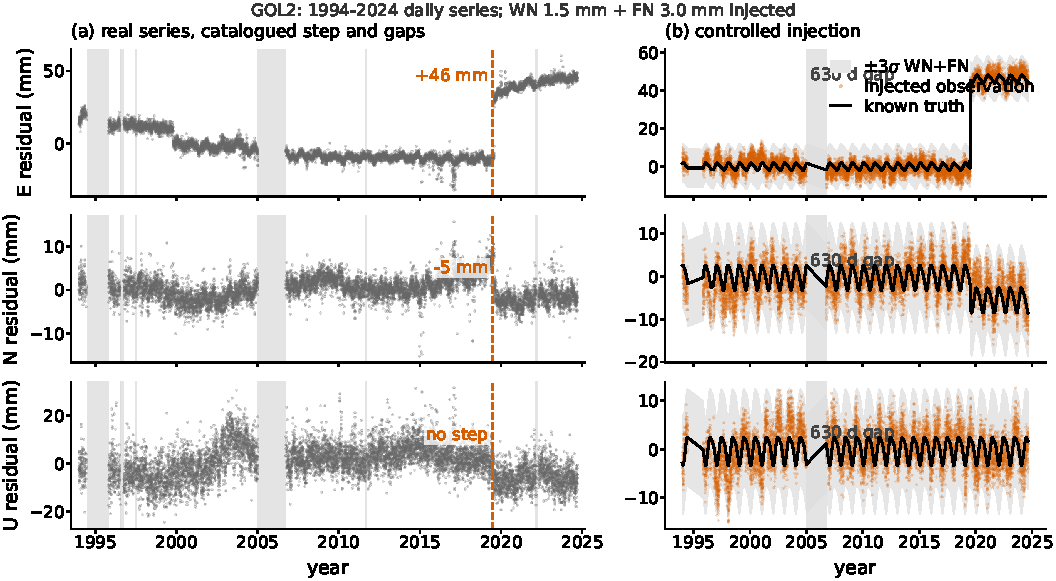
\includegraphics[width=\linewidth]{figures/fig02_real_sample.pdf}
\caption{The benchmark works on real series with known injected noise.
(a) Residuals of the three components of a held-out NGL station after removing a
robust trend; the dashed line marks the catalogued discontinuity and the shaded
bands the observation gaps. (b) The same station after controlled injection of
white (1.5~mm) and flicker (3.0~mm) noise, with the exact truth in black, the
injected observation in orange and the $\pm3\sigma$ noise envelope; the largest
gap is retained. Because the truth is known at every epoch, recovery error needs
no proxy.}
\label{fig:sample}
\end{figure}

The NGL subset is a deterministic function of the NGL station holdings, frozen so
that the selection is reproducible. A station is eligible if it has at least
4000 solutions, begins no later than 2009, continues to at least 2024 and spans
at least 15 years; the 300 eligible stations with the longest records are taken,
ties broken by solution count and site code. After quality control (at least 600
epochs, daily completeness at least 0.5, span at least 5 years) 298 NGL series
remain. Record spans run from 5.87 to 30.64 years with a median of 30.03 years,
daily completeness from 0.500 to 0.997 with a median of 0.972, and the combined
time span is 1994.00--2024.65. The station list and the catalogue hash are part of
the release, so the selection can be reproduced exactly.

\paragraph{Station-level split.}
The 60/20/20 split is drawn by site, not by epoch: all series of a site fall in
the same fold, and a site present in both sources stays together. The folds hold
198, 68 and 67 series, corresponding to 193, 64 and 64 sites, with 1\,907\,614,
651\,833 and 647\,892 daily epochs. Only the test fold is scored. The test fold
contains 61 NGL series and 6 JPL series from distinct sites; the JPL arm is
therefore small but genuinely held out by site. The validation fold is used to
choose the fixed training budget and, where stated, the read-out threshold; it is
never scored. Fig.~\ref{fig:split} shows the split geography, counts and record
lengths; the three folds are comparable in span, and no site crosses a fold.

\begin{figure}[t]
\centering
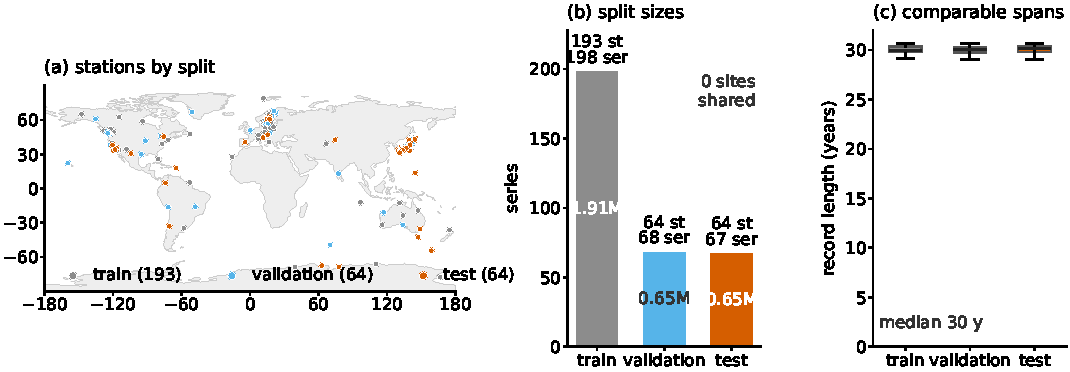
\includegraphics[width=\linewidth]{figures/fig04_split.pdf}
\caption{The split is drawn by site, not by epoch. (a) Held-out sites cover all
five regions and both analysis centres; (b) the three folds hold 193, 64 and 64
sites (198, 68 and 67 series) with zero sites shared; (c) the folds have
comparable record lengths (median about 30 years). Because every series of a
site stays in one fold, a learned method cannot memorise a station in training
and be scored on another component or source of the same station.}
\label{fig:split}
\end{figure}

\paragraph{Real discontinuity labels.}
For the real-label detection task we use the NGL discontinuity catalogue
(\url{https://geodesy.unr.edu/NGLStationPages/steps.txt}, downloaded
2026-10-18; 142\,625 lines; catalogue sha256
\texttt{\seqsplit{49894f7566ed34da3eb646087fc2fc64c5766720ba2368a3f6f6df53f3f282d8}}).
Two codes are retained: code 1, equipment change, and code 2, possible earthquake
step. A label is kept for a component only when its catalogued date lies inside
the record with a 0.5-year margin, its observed level change is at least three
times the local noise scale, and no other kept label lies within 60 days. This
yields 1\,743 labels on 153 component series from 58 held-out stations. The
labels are dominated by code 2 (1\,691 of 1\,743), so the real-label task
measures detection of earthquake-related steps more than of equipment changes;
we state this as a property of the data, not as a claim about all offsets. The
catalogue dates are not adjusted for post-seismic transients, which contributes
to the detection delay measured in Sec.~\ref{sec:results:t3:real}.

\paragraph{External and regional arms.}
Held-out JPL sites form the external arm: the six test JPL series are scored
separately from the 61 NGL series by the same methods. As a regional check we
also group the test sites into five geographic regions (Europe, North America,
Asia, Pacific and other) and report per-region scores (Fig.~\ref{fig:map}).
Neither arm changes any training or threshold decision.

\begin{figure}[t]
\centering
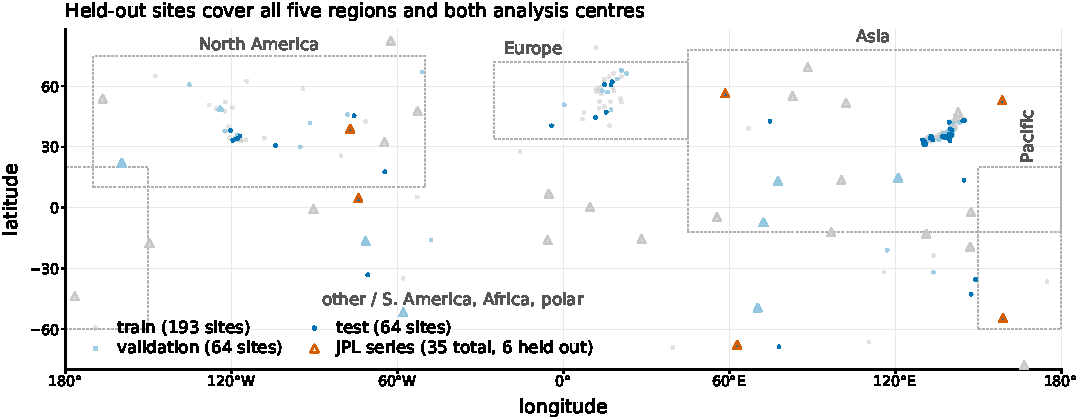
\includegraphics[width=\linewidth]{figures/fig11_map.pdf}
\caption{Geographic coverage of the split. Held-out (orange) sites fall in all
five scoring regions and include both NGL and JPL series, so the regional and
external arms test the same frozen networks outside the training geography
rather than a single continent. The map is descriptive; it enters no training or
threshold decision.}
\label{fig:map}
\end{figure}

\paragraph{Noise levels.}
The injected noise in the primary experiments is white noise with
$\sigma_{\rm WN}=1.5$~mm plus flicker noise with $\sigma_{\rm FN}=3.0$~mm. The
random-walk arm adds $\sigma_{\rm RW}=1.0$~mm. These levels were fixed before
any task was run. As a check on where they sit, we applied Whittle MLE to the
robust trajectory residual of all 999 component series in the benchmark: the
median white-noise level is 1.90~mm (interquartile range 1.39--3.67) and the
median flicker level 2.26~mm (1.61--5.74). The injected white level therefore
lies near the lower quartile and the flicker level inside the central half of
the empirical distribution (Fig.~\ref{fig:station_noise}). The recovered
random-walk median is 10.29~mm\,yr$^{-1/2}$, but that estimate absorbs
unmodelled transients and is an upper bound; the injected 1.0~mm\,yr$^{-1/2}$
is below it, so the random-walk arm is a sensitivity test rather than a
calibrated replay of the stations' noise.

\begin{figure}[t]
\centering
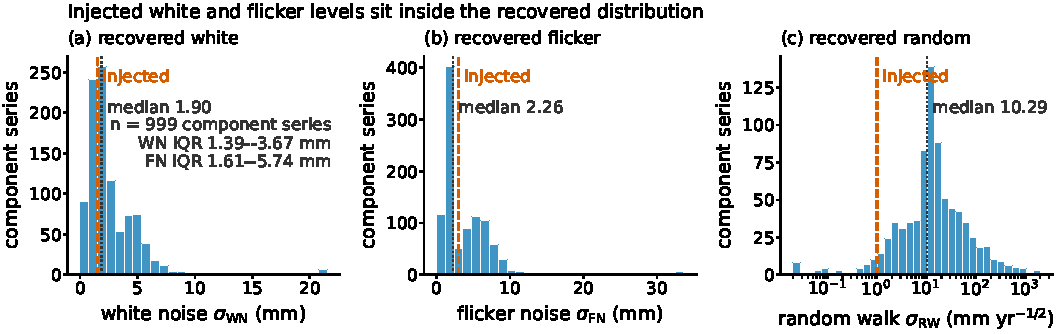
\includegraphics[width=\linewidth]{figures/fig14_station_noise.pdf}
\caption{Whittle estimates on the robust residual of every benchmark series.
The recovered white-noise distribution has a median of 1.90~mm (interquartile
range 1.39--3.67) and the recovered flicker distribution a median of 2.26~mm
(1.61--5.74); the injected levels (1.5 and 3.0~mm, dashed) sit near the lower
quartile and inside the central half, respectively. The random-walk estimate is
an upper bound because transients are absorbed by that component, which is why
the random-walk arm is a sensitivity test.}
\label{fig:station_noise}
\end{figure}
